\documentclass[11pt]{article}
\usepackage[margin=0.85in]{geometry}
\usepackage[T1]{fontenc}
\usepackage{lmodern}
\usepackage{microtype}
\usepackage{parskip}
\usepackage{graphicx}
\usepackage{xcolor}
\usepackage{hyperref}
\usepackage{enumitem}

\definecolor{Ink}{HTML}{1F2937}
\definecolor{Muted}{HTML}{6B7280}
\definecolor{Teal}{HTML}{147A73}

\hypersetup{
  colorlinks=true,
  linkcolor=Teal,
  urlcolor=Teal
}

\setlist[itemize]{topsep=4pt,itemsep=4pt,leftmargin=1.3em}

\title{General Field Presentation\\Recommended Figures Pack}
\author{Sahara Kaul \and Kelsey Pattison \and Ahmed Sajid}
\date{CMPUT 414, Winter 2026}

\begin{document}
\color{Ink}
\maketitle
\tableofcontents
\newpage

\section{How To Use This Pack}

This document collects paper figures that are likely to be useful in the current general field presentation. For each figure, the goal is to answer three questions:

\begin{itemize}
\item where it should go in the presentation,
\item what idea it helps explain,
\item and what the original source is.
\end{itemize}

These are not meant to be the only visuals in the slide deck. They are the paper-derived figures that are most worth borrowing because they add explanatory value.

\section{WaveGAN: Phase Shuffle / Raw Audio GANs}

\begin{center}
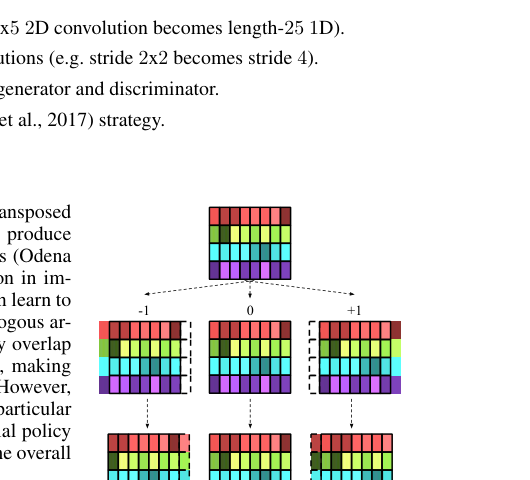
\includegraphics[width=0.82\linewidth]{figure_pack/crops/wavegan_phase_shuffle.png}
\end{center}

\textbf{Use it for}\\
The \emph{WaveGAN} slide, especially when explaining why audio GANs needed tricks like phase shuffle.

\textbf{Why it helps}\\
This figure is visually memorable and gives a concrete picture of how the phase-shuffle idea perturbs discriminator feature maps. It makes the point that raw audio GANs were not just about copying image GANs directly; they needed audio-specific adjustments.

\textbf{Source}\\
Donahue, McAuley, and Puckette, \emph{Adversarial Audio Synthesis}, ICLR 2019, Figure 3.\\
\url{https://arxiv.org/abs/1802.04208}

\newpage
\section{MoVE: Many-to-Many Timbre Transfer Architecture}

\begin{center}
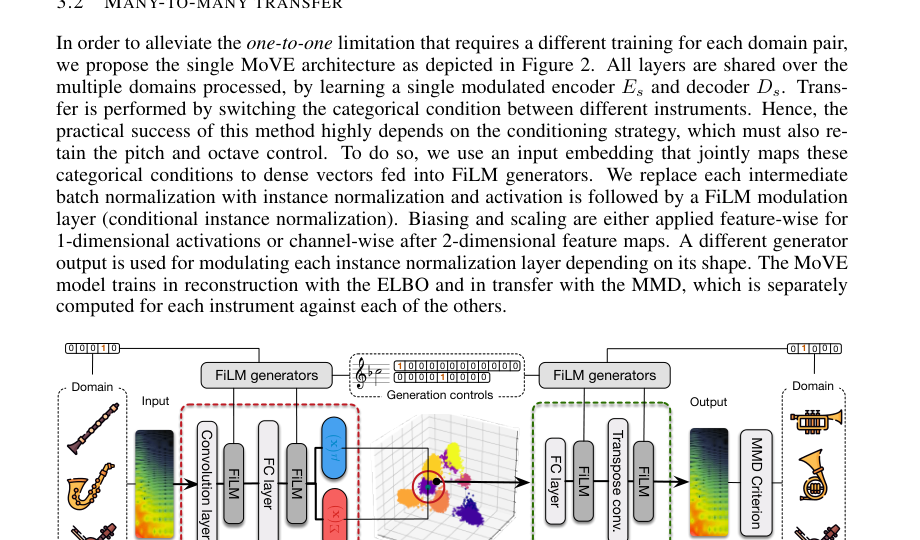
\includegraphics[width=0.88\linewidth]{figure_pack/crops/move_architecture.png}
\end{center}

\textbf{Use it for}\\
The \emph{MoVE} slide in the latent structured audio section.

\textbf{Why it helps}\\
This is one of the most useful architecture figures in the whole talk because it shows, in one place, why MoVE is more transfer-specific than a generic VAE. You can literally point to the FiLM generators and the many-to-many domain setup while talking.

\textbf{Source}\\
Bitton, Esling, and Chemla-Romeu-Santos, \emph{Modulated Variational auto-Encoders for Many-to-Many Musical Timbre Transfer}, Figure 2.\\
\url{https://arxiv.org/abs/1810.00222}

\newpage
\section{RAVE: Fidelity / Reconstruction Tradeoff}

\begin{center}
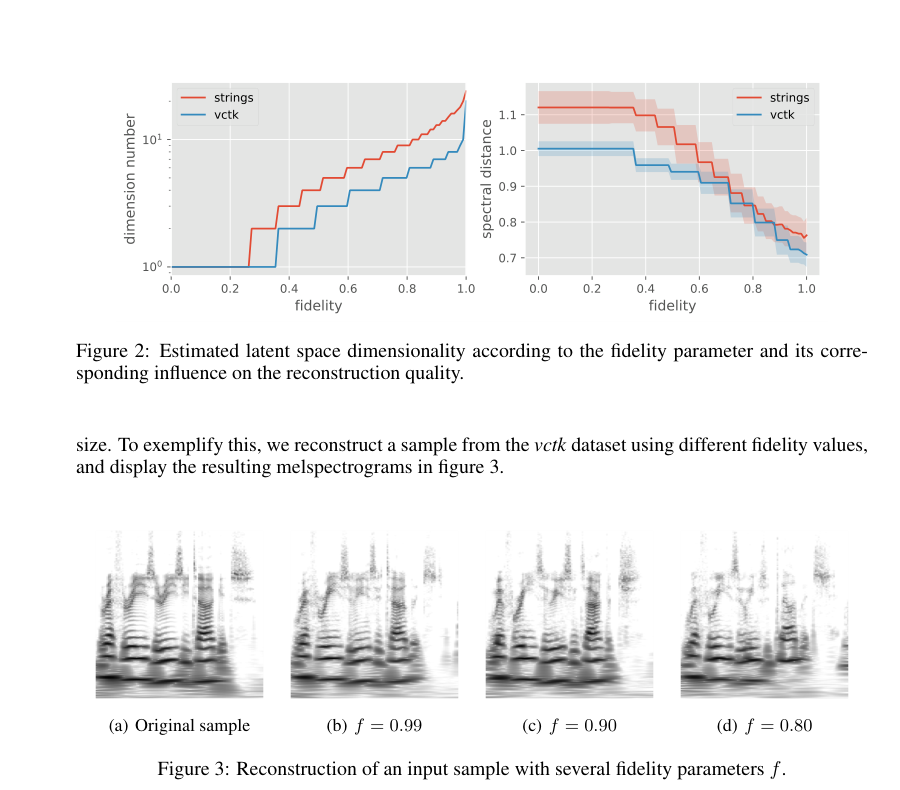
\includegraphics[width=0.82\linewidth]{figure_pack/crops/rave_reconstruction.png}
\end{center}

\textbf{Use it for}\\
The \emph{RAVE} slide, especially if you keep RAVE as a short ``practical latent audio'' bridge.

\textbf{Why it helps}\\
This crop shows that RAVE is really about practical latent audio compression and reconstruction quality. It is useful if you want to explain that RAVE is less about perfect disentanglement and more about making latent audio good enough to manipulate and resynthesize.

\textbf{Source}\\
Caillon and Esling, \emph{RAVE: A variational autoencoder for fast and high-quality neural audio synthesis}, Figures 2 and 3 area.\\
\url{https://arxiv.org/abs/2111.05011}

\newpage
\section{BigVGAN: Architecture Overview}

\begin{center}
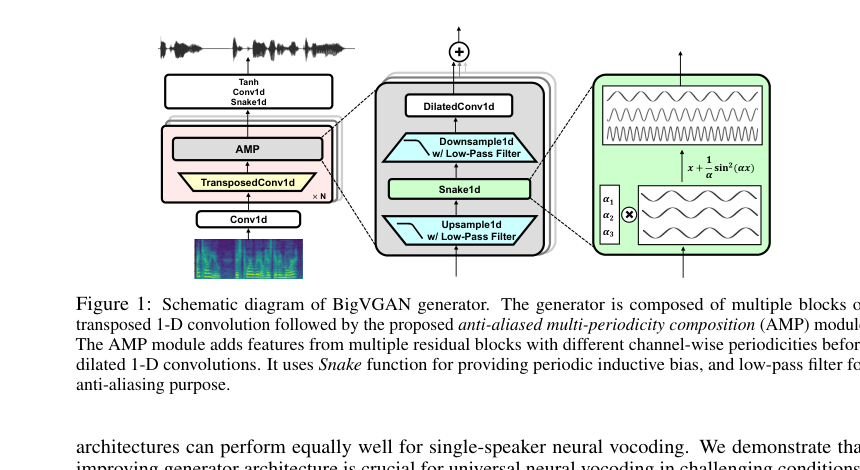
\includegraphics[width=0.82\linewidth]{figure_pack/crops/bigvgan_architecture.png}
\end{center}

\textbf{Use it for}\\
The \emph{BigVGAN} slide in the modern controllable synthesis section.

\textbf{Why it helps}\\
This figure gives a clean visual explanation of the AMP module, the Snake activation, and the audio-specific inductive bias that makes BigVGAN more than just ``another vocoder.'' If you are only going to show one BigVGAN visual, this is the right one.

\textbf{Source}\\
Lee et al., \emph{BigVGAN: A Universal Neural Vocoder with Large-Scale Training}, Figure 1.\\
\url{https://arxiv.org/abs/2206.04658}

\newpage
\section{DDPM: Graphical Model / Forward-Reverse Process}

\begin{center}
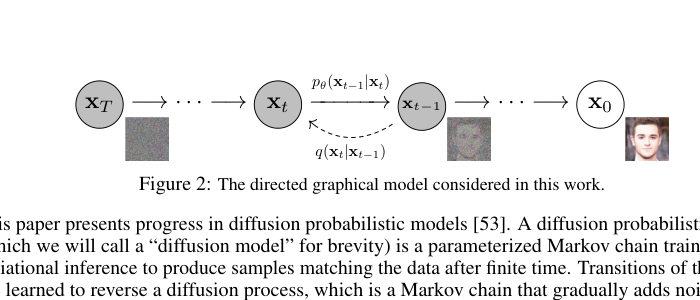
\includegraphics[width=0.76\linewidth]{figure_pack/crops/ddpm_graphical_model.png}
\end{center}

\textbf{Use it for}\\
The \emph{DDPM} slide.

\textbf{Why it helps}\\
This is probably the cleanest figure to use when introducing diffusion at a high level. It gives the audience a visual model of the forward noising chain and the learned reverse denoising chain without needing to dwell too much on the math.

\textbf{Source}\\
Ho, Jain, and Abbeel, \emph{Denoising Diffusion Probabilistic Models}, Figure 2.\\
\url{https://arxiv.org/abs/2006.11239}

\newpage
\section{Classifier-Free Guidance: Guidance Strength Examples}

\begin{center}
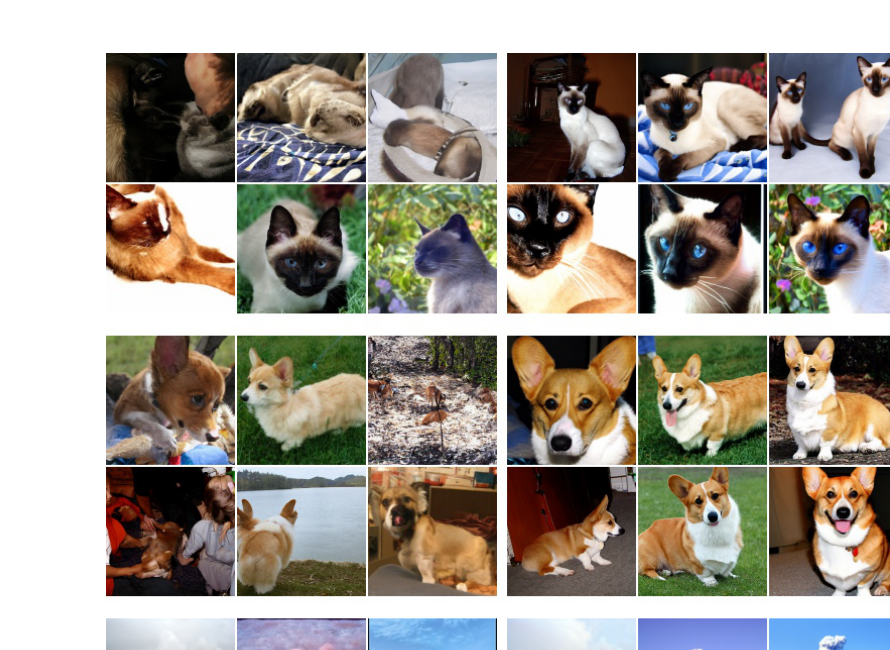
\includegraphics[width=0.82\linewidth]{figure_pack/crops/cfg_guidance_examples.png}
\end{center}

\textbf{Use it for}\\
The \emph{Classifier-Free Guidance} slide.

\textbf{Why it helps}\\
This figure is visually strong because it lets the audience see the effect of stronger guidance immediately. Even though the domain is images, the conceptual point carries over well: larger guidance pushes harder toward the condition, sometimes at the expense of diversity or naturalness.

\textbf{Source}\\
Ho and Salimans, \emph{Classifier-Free Diffusion Guidance}, Figure 3.\\
\url{https://arxiv.org/abs/2207.12598}

\newpage
\section{SDEdit: Source-Preserved Editing Process}

\begin{center}
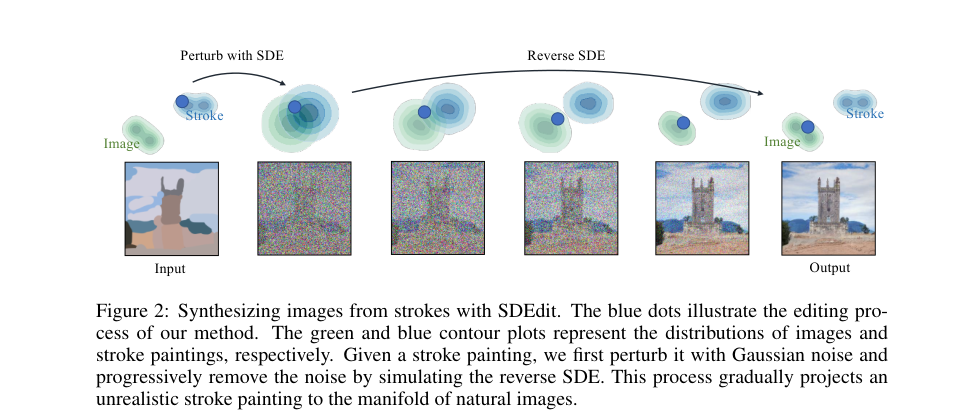
\includegraphics[width=0.84\linewidth]{figure_pack/crops/sdedit_overview.png}
\end{center}

\textbf{Use it for}\\
The \emph{SDEdit} slide.

\textbf{Why it helps}\\
This is one of the best figures in the pack because it visually explains the whole idea of SDEdit in one line: perturb the source with noise, then reverse the diffusion process into a more realistic output. It directly supports your point about preserving a source skeleton while still allowing meaningful change.

\textbf{Source}\\
Meng et al., \emph{SDEdit: Guided Image Synthesis and Editing with Stochastic Differential Equations}, Figure 2.\\
\url{https://arxiv.org/abs/2108.01073}

\newpage
\section{AudioLDM: Audio Manipulation by Latent Diffusion}

\begin{center}
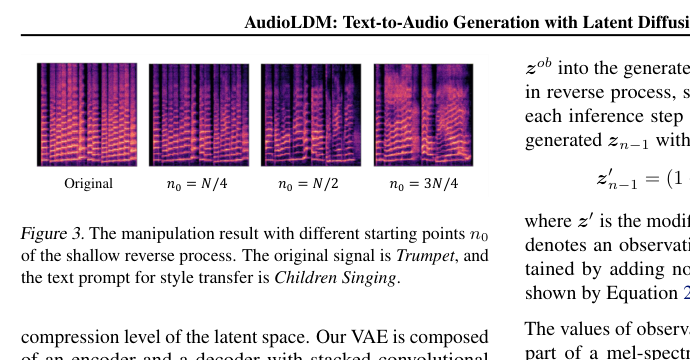
\includegraphics[width=0.82\linewidth]{figure_pack/crops/audioldm_manipulation.png}
\end{center}

\textbf{Use it for}\\
The \emph{AudioLDM} slide.

\textbf{Why it helps}\\
This is probably the most directly relevant modern figure for your final section. It shows that AudioLDM is not only about generation from scratch; it also supports manipulation starting from an existing audio source. That aligns very closely with your genre-remastering story.

\textbf{Source}\\
Liu et al., \emph{AudioLDM: Text-to-Audio Generation with Latent Diffusion Models}, Figure 3.\\
\url{https://arxiv.org/abs/2301.12503}

\newpage
\section{Best Shortlist}

If you only use a few paper figures, the most useful shortlist is:

\begin{itemize}
\item \textbf{MoVE architecture} for the latent-transfer section.
\item \textbf{DDPM graphical model} for the first diffusion slide.
\item \textbf{SDEdit overview} for the editing / source-anchoring slide.
\item \textbf{AudioLDM manipulation figure} for the modern audio-diffusion slide.
\item \textbf{CFG guidance examples} if you want one visually obvious control example.
\end{itemize}

If you want a slightly larger set, add:

\begin{itemize}
\item \textbf{WaveGAN phase-shuffle figure} for historical context.
\item \textbf{BigVGAN architecture} for realism / vocoder explanation.
\item \textbf{RAVE reconstruction figure} if you keep RAVE in the deck.
\end{itemize}

\end{document}
